%
% Copyright (c) 2017  Pavel Kirienko <pavel.kirienko@zubax.com>
%

\documentclass{zubaxdoc}
\graphicspath{{document_templates/documentation_template_latex/}}

\usepackage{xstring}
\usepackage{multirow}
\usepackage{diagbox}

\title{Sapog v2 Reference Manual}

%
% Use this macro to define configuration parameter names.
% It automatically creates parameter references that can be accessed later using the respective macro.
% Note that underscores in the parameter name must be replaced with +, e.g.:
%   \CfgDef{mot+abc+def}
% Expands to:
%   mot_abc_def
%
% TODO: We may want to add an index of configuration parameters at the end of the document?
%       It would be quite easy to do with this macro.
%
\newcommand{\CfgDef}[1]{
    \StrSubstitute{#1}{+}{\textunderscore}[\temp]
    \texttt{\temp}\label{#1}
}

%
% Use this macro to refer to configuration parameter definition from other parts of the document.
% Note that underscores in the parameter name must be replaced with +, e.g.:
%   \CfgRef{mot+abc+def}
% Expands to:
%   mot_abc_def
%
\newcommand{\CfgRef}[1]{
    \StrSubstitute{#1}{+}{\textunderscore}[\temp]
    % It is also possible to create a reference with custom text using \hyperref[]{}, but that seems excessive.
    \texttt{\temp} {\footnotesize (page \pageref{#1})}
}

\begin{document}
\frontmatter

\begin{titlepage}
\section*{Overview}

Sapog is an advanced open source sensorless PMSM/BLDC motor controller firmware designed for
use in propulsion systems of electric unmanned aircraft and watercraft.

The source repository and the public bug tracker are located at
\url{https://github.com/PX4/sapog}.

This document is applicable to firmware versions 2.x released until \today.

This document focuses only on the firmware.
Please refer to your product documentation for relevant information about the hardware.

\section*{Applications}
\begin{itemize}
    \item Propeller drives of unmanned aerial vehicles.
    \item Watercraft propulsion systems.
    \item General purpose sensorless BLDC drives.
\end{itemize}

\BeginRightColumn
\section*{Features}
\begin{itemize}
    \item Robust motor control and resilience to synchronization losses in all operating modes.
    \item Fast response. This feature is especially critical for multirotor aircraft.
    \item Regenerative braking and active freewheeling.
    \item Optional RPM control loop (RPM governor).
    \item Current limiting.
    \item Self diagnostics and extensive real-time status reporting.
    \item Compatible with most BLDC motors with very little tuning.
    \item Highly configurable.
    \item Automatic firmware update over UAVCAN in the field.
    \item Supported communication interfaces:
    \begin{itemize}
        \item UAVCAN interface with optional double redundancy.
        \item Command line interface over UART, suitable for M2M communications.
        \item RCPWM (analog PWM interface widely used in robotics).
    \end{itemize}
\end{itemize}

\end{titlepage}

\tableofcontents
\listoffigures
\listoftables

\mainmatter

\chapter{Principles of operation}

This chapter provides a brief overview of the basic operating principles of electric permanent magnet
synchronous motors, and the relevant approaches and solutions implemented in Sapog.

\section{Definitions}

\begin{description}
    \item[PMSM] Permanent magnet synchronous motor.
    \item[BLDC] Brushless DC motor.
    \item[RPM] Revolutions per minute.
    \item[EMF] Electromotive force.
    \item[BEMF] Back electromotive force.
    \item[$K_V$] Motor velocity constant. Sometimes written as KV, although
    this form is discouraged because it can be confused with kilovolt.
\end{description}

\section{PMSM and BLDC motors}

\subsection{Basic equations}\label{sec:motor_equations}

This section provides the most important equations that describe a DC electric motor.
The principles explained here can be extended to all types of polyphase PMSM motors as well.

In the context of electric drives, BEMF is the voltage induced on the motor windings
while the armature of the motor is moving relative to the magnetic field of the rotor.
The induced voltage can be observed on the phase leads of the motor.
The magnitude of the induced voltage is dependent on the speed of the armature relative to the magnetic field
of the rotor, and the magnetic flux linkage of the motor. The dependency can be expressed as follows:
\begin{equation}
E_b = \phi \omega_e
\end{equation}
where $E_b$ is the induced back electromotive force, $\phi$ is the magnetic flux linkage,
and $\omega_e$ is the electrical angular velocity.

Electrical angular velocity $\omega_e$ is a function of the mechanical angular velocity $\omega_m$
and the number of rotor magnetic poles $N_p$:
\begin{equation}
\omega_e = \frac{2 \omega_m}{N_p}\qquad
N_p \geq 2, N_p\text{\ is even}
\end{equation}

Both mechanical and electrical angular velocity are related to the mechanical and electrical RPM,
respectively, as follows:
\begin{equation}
\text{RPM} = \frac{30 \omega }{\pi }
\end{equation}

Motor velocity constant $K_V$ can be expressed via the magnetic flux linkage $\phi$ as follows:
\begin{equation}
K_V = \frac{20 \sqrt{3}}{\pi  N_p \phi }
\end{equation}

The armature current $I_a$ is proportional to the voltage difference between the induced back EMF and
the source voltage $E_s$:
\begin{equation}
I_a = \frac{E_s - E_b}{R}
\end{equation}
where $R$ is the internal resistance of the stator.

Torque $\tau$ observed on the shaft is dependent on the torque-generating current and the velocity constant
as follows:
\begin{equation}
\tau = \frac{30 I_a}{\pi K_V}
\end{equation}

The mechanical power output $P$ is the product of the torque and the mechanical angular velocity:
\begin{equation}
P = \tau \omega_m
\end{equation}

\subsection{BEMF shape}

There are two major types of permanent magnet synchronous motors (PMSM) that differ by the shape of the back
electromotive force induced while the rotor is moving at a constant speed.

The first type has a fixed magnetic flux linkage that is independent of the electrical position of the rotor.
The induced BEMF per phase therefore has a sinusoidal shape.
These motors are typically referred to simply as PMSM, or BLAC.
Since the term PMSM is quite ambiguous, we will be using the term BLAC to refer to a PMSM with sine shaped BEMF.

The other type, referred to as brushless DC, or BLDC, has a variable flux linkage that changes with the
rotor position in a specific way that results in the trapezoidal shape of the back EMF.
The difference is illustrated on the figure \ref{bemf_trapezoidal_vs_sinusoidal}.

\begin{figure}[hbt]
    \centering
	\includegraphics[width=0.6\textwidth]{bemf_trapezoidal_vs_sinusoidal}
	\caption{Difference between trapezoidal and sinusoidal BEMF.
	\label{bemf_trapezoidal_vs_sinusoidal}}
\end{figure}

Sapog, being a BLDC drive, drives the motor with trapezoidal modulated voltage.
This produces smooth torque and vibration free operation with BLDC motors,
since it is expected that the flux linkage will be changing in a specific way.

Like any BLDC drive, Sapog can operate with BLAC motors as well, albeit with increased torque ripple.
From the model presented in section \ref{sec:motor_equations} we can predict that the motor
will exhibit periodic variations in the output torque if the form of the voltage modulated by the controller
does not match with the form of the back EMF induced in the motor.
The resulting periodic torque variations that occur in a BLAC motor driven by a BLDC drive
(and, likewise, in a BLDC motor driven with sine modulated voltages) are shown on the figure 
\ref{sine_torque_deviation}.

\begin{figure}[hbt]
    \centering
	\includegraphics[width=0.6\textwidth]{sine_torque_deviation}
	\caption{Torque ripple caused by mismatching forms of the back EMF and the source voltage.
	\label{sine_torque_deviation}}
\end{figure}

Many applications, however, can tolerate the induced torque ripple and associated vibrations produced
by the motor.

\section{BLDC basics}

\subsection{Commutation sequence}

\newcommand{\BEMFH}{$\uparrow$}
\newcommand{\BEMFL}{$\downarrow$}

Three phase BLDC drives operate by modulating a specific sequence of voltages on the motor phases
synchronously with the movement of the rotor.
The modulated voltage sequences are shown in the commutation table below
(legend: $+$ -- positive voltage output; $-$ -- negative voltage output;
\BEMFH{} -- the phase is floating, induced BEMF is rising;
\BEMFL{} -- the phase is floating, induced BEMF is falling).

\begin{tabu}{|l c|c c c c c c|}
    \hline
    \rowfont{\bfseries}
    \multicolumn{2}{|c|}{\diagbox{Phase}{Step}}
                                 & 0     & 1     & 2     & 3     & 4     & 5     \\\hline
    \multirow{3}{*}{Forward} & A & $-$   &\BEMFH & $+$   & $+$   &\BEMFL & $-$   \\
                             & B & $+$   & $+$   &\BEMFL & $-$   & $-$   &\BEMFH \\
                             & C &\BEMFL & $-$   & $-$   &\BEMFH & $+$   & $+$   \\\hline
    \multirow{3}{*}{Reverse} & A & $-$   &\BEMFH & $+$   & $+$   &\BEMFL & $-$   \\
                             & B &\BEMFL & $-$   & $-$   &\BEMFH & $+$   & $+$   \\
                             & C & $+$   & $+$   &\BEMFL & $-$   & $-$   &\BEMFH \\\hline
\end{tabu}

The rotor position is deduced from the behavior of the induced BEMF on the floating phase.
From figure \ref{bemf_trapezoidal_vs_sinusoidal} we can deduce that when the induced BEMF of the floating
phase crosses the median voltage between the high and the low phase, there is 30 electrical degrees left
before the next commutation step begins.
The controller employs this rule to estimate the time when the next commutation should occur.
The process is demonstrated on the figure \ref{commutation_basics}.
The voltage waveforms shown on the figure were acquired from the phase voltage signal conditioning circuits,
before the ADC inputs, shown on the figure \ref{power_stage_schematic}.

\begin{figure}[hbt]
    \centering
	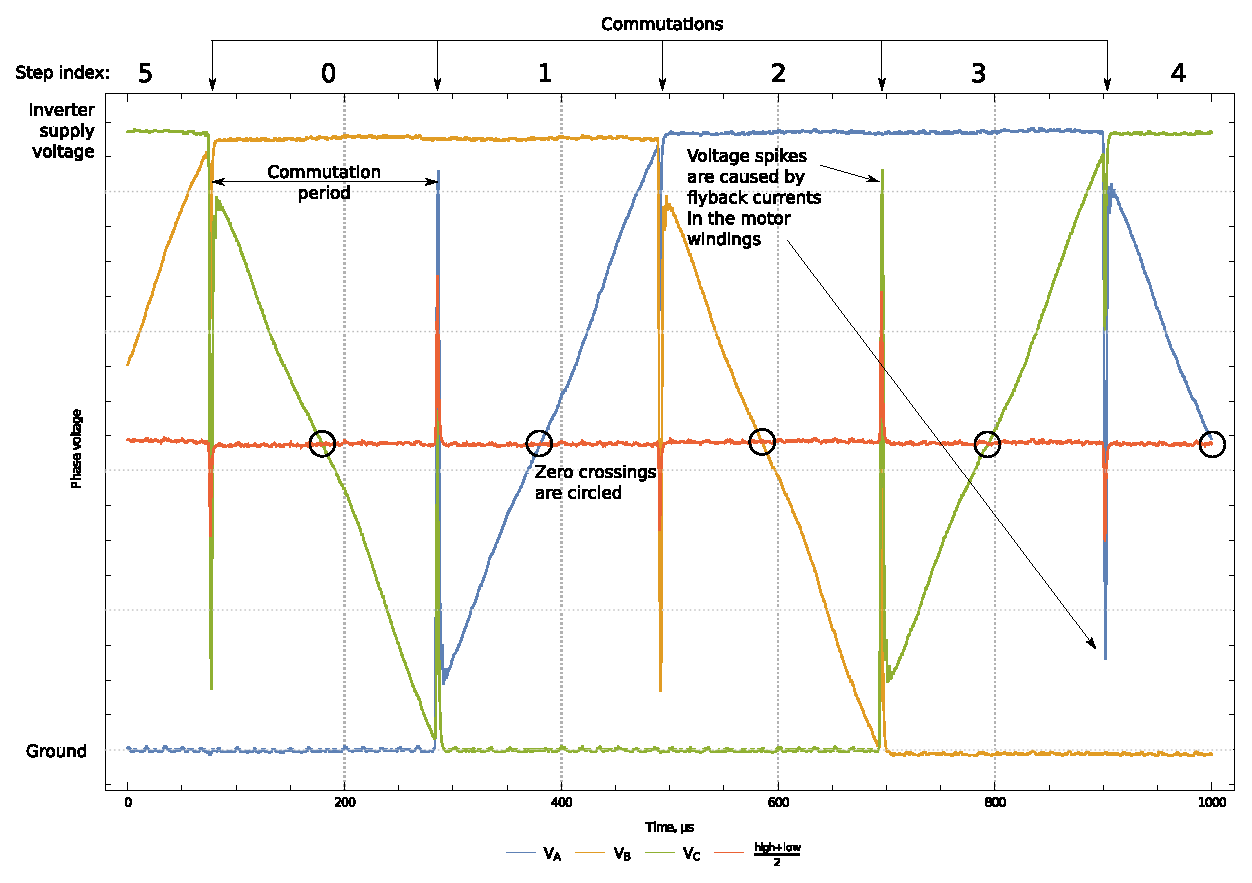
\includegraphics[width=\textwidth]{commutation_basics}
	\caption{Six step commutation sequence observed through phase voltages.
	\label{commutation_basics}}
	PWM modulation is not seen because the shown voltages were acquired while the controller
	was operating at full duty cycle.
\end{figure}

\begin{figure}[hbt]
    \centering
	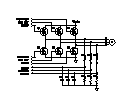
\includegraphics[width=\textwidth]{power_stage_schematic}
	\caption{Simplified schematic of the power stage design that Sapog relies on.
	\label{power_stage_schematic}}
\end{figure}

From the section \ref{sec:motor_equations} we know that the magnitude of the induced BEMF is linearly
dependent on the speed of relative motion between the armature and the rotor magnetic field.
Considering also the fact that the controller relies on the induced BEMF signal for rotor position estimation,
we can predict that the rotor position estimation may be unreliable if the induced BEMF is not sufficiently
high. In order to avoid issues at low speed operation, Sapog provides several configuration parameters that
restrict the minimum operating speed, such as the following:

\begin{itemize}
\item \CfgRef{mot+comm+per+max} - maximum commutation period. The estimated commutation period
will be artificially constrained to not exceed this value.
\item \CfgRef{mot+rpm+min} - minimum RPM that can be demanded in RPM governor mode.
If the demanded RPM is lower, the setpoint will be artificially increased.
\item \CfgRef{mot+v+min} - minimum source voltage when operating in open loop mode.
If the demanded duty cycle amounts to a lower source voltage than this, the setpoint will be artificially
increased.
\end{itemize}

\subsection{Field weakening}

From section \ref{sec:motor_equations} we know that the maximum speed that a motor can achieve is dependent
on the the load, magnetic flux linkage, and the source voltage.
Reduction of the magnetic flux linkage decreases the induced BEMF, which allows the rotor reach higher speed,
given constant source voltage and load.

The controller can alter the commutation sequence in a specific way, causing the rotating magnetic field
created by the stator to interact with the magnetic field of the rotor in a way that reduces the magnetic
field linkage, effectively increasing the maximum speed of the rotor, reducing the output torque,
while keeping the maximum mechanical power output constant.
Note that since part of the energy is expended on suppression of the magnetic fields induced by the rotor,
the overall efficiency of the drive decreases with higher field weakening.

This technique is known as \emph{field weakening}, and it is implemented by means of adjustment of the 
commutation sequence, shortening the time interval from the zero crossing point to the moment when the next
commutation step begins.
In the context of BLDC drives this specific approach is also known as \emph{commutation advancing}.

Sapog defines commutation advance angle in electrical angular degrees of rotor position,
and it can vary from 0\degree{} to 29\degree{}, inclusively, where 0\degree{} corresponds to no advance,
and 29\degree{} corresponds to the maximum advance angle.
The practical effects imposed on the drive are summarized in the following table.

\begin{ZubaxCompactTable}{|c|c c c c|}
    Advance angle & Flux linkage & Maximum torque & Maximum speed & Drive efficiency \\
    Low           & High         & High           & Low           & High             \\
    High          & Low          & Low            & High          & Low              \\
\end{ZubaxCompactTable}

Sapog can modulate a fixed advance angle, or it can be defined as a function of speed.
The latter is especially useful, since high field weakening at low speeds does not make practical sense,
and serves only to reduce the drive efficiency with no apparent benefit to the application.
Additionally, high field weakening may be responsible for stability issues at low operating speeds,
because it effectively reduces the magnitude of the BEMF induced in the motor.

The field weakening feature is configured with the help of the following configuration parameters:

\begin{itemize}
\item \CfgRef{mot+tim+adv+max} - maximum commutation advance angle.
\item \CfgRef{mot+tim+adv+min} - minimum commutation advance angle.
\item \CfgRef{mot+tim+cp+min} - when the current commutation period is longer than this value,
the minimum advance angle will be used.
\item \CfgRef{mot+tim+cp+max} - when the current commutation period is shorter than this value,
the maximum advance angle will be used.
\end{itemize}

When the current commutation period is between \verb|mot_tim_cp_max| and \verb|mot_tim_cp_min|,
the advance angle will be proportionally linearly interpolated between
\verb|mot_tim_adv_min| and \verb|mot_tim_adv_max|.
The interpolation logic is demonstrated on the figure \ref{timing_advance_interpolation_plot}.

\begin{figure}[hbt]
    \centering
	\includegraphics[width=0.6\textwidth]{timing_advance_interpolation_plot}
	\caption{Timing advance interpolation logic.
	\label{timing_advance_interpolation_plot}}
\end{figure}

Sample phase voltage waveforms acquired while the controller was operating under high field
weakening settings are shown on the figure \ref{phase_voltages_at_high_advance_angle}.

\begin{figure}[hbt]
    \centering
	\includegraphics[width=\textwidth]{phase_voltages_at_high_advance_angle}
	\caption{Commutation sequence at high advance angle settings.
	\label{phase_voltages_at_high_advance_angle}}
	It can be seen that the next commutation begins shortly after the induced BEMF
	crosses the neutral voltage.
\end{figure}

\subsection{Rotor position observer}

\subsection{Spin-up}



\chapter{Configuration parameters}

\CfgDef{esc+index}
\CfgDef{cmd+ttl+ms}
\CfgDef{cmd+start+dc}
\CfgDef{uavcan+node+id}
\CfgDef{light+index}
\CfgDef{pwm+max+usec}
\CfgDef{pwm+min+usec}
\CfgDef{pwm+enable}
\CfgDef{enum+max+step}
\CfgDef{enum+steps}
\CfgDef{enum+bemf}
\CfgDef{mot+pwm+dt+ns}
\CfgDef{mot+pwm+hz}
\CfgDef{mot+spup+blnk+pm}
\CfgDef{mot+spup+to+ms}
\CfgDef{mot+spup+st+cp}
\CfgDef{mot+comm+per+max}
\CfgDef{mot+zc+fails+max}
\CfgDef{mot+bemf+range}
\CfgDef{mot+bemf+win+den}
\CfgDef{mot+blank+usec}
\CfgDef{mot+tim+cp+min}
\CfgDef{mot+tim+cp+max}
\CfgDef{mot+tim+adv+max}
\CfgDef{mot+tim+adv+min}
\CfgDef{mot+i+shunt+mr}
\CfgDef{rpmctl+i}
\CfgDef{rpmctl+d}
\CfgDef{rpmctl+p}
\CfgDef{mot+stop+thres}
\CfgDef{mot+lpf+freq}
\CfgDef{mot+i+max+p}
\CfgDef{mot+i+max}
\CfgDef{mot+rpm+min}
\CfgDef{ctl+dir}
\CfgDef{mot+num+poles}
\CfgDef{mot+dc+slope}
\CfgDef{mot+dc+accel}
\CfgDef{mot+spup+vramp+t}
\CfgDef{mot+v+spinup}
\CfgDef{mot+v+min}

\end{document}
